\newpage
\appendix
\section{Appendix}
\subsection{Figures and graphs}

\subsubsection{The ``Bump'' Function}\label{app:bump_function}
\begin{figure}[H]
    \centering
    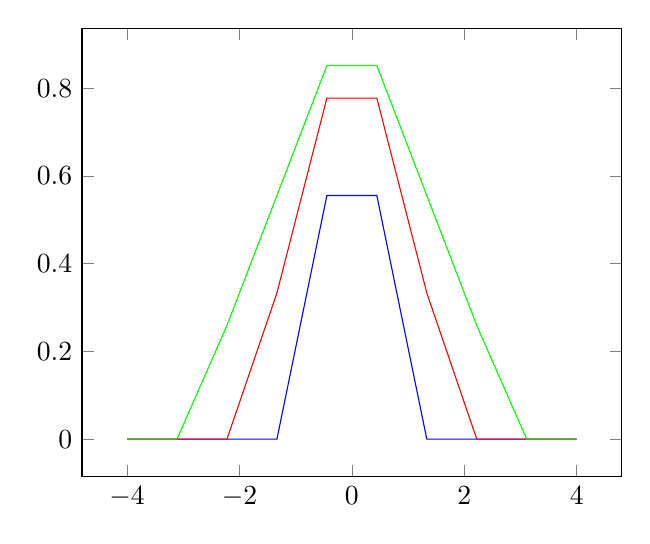
\begin{tikzpicture}
    \begin{axis}
    \addplot[domain=-4:4, samples=10, color=blue,]{max(x-1,0) + max(x+1,0) - 2*max(x,0)};
    \addplot[domain=-4:4, samples=10, color=red,]{max(x/2-1,0) + max(x/2+1,0) - 2*max(x/2,0)};
    \addplot[domain=-4:4, samples=10, color=green,]{max(x/3-1,0) + max(x/3+1,0) - 2*max(x/3,0)};
    \end{axis}
\end{tikzpicture}
    \caption{Illustration of the so-called ``bump'' function $\psi_a(x)$ used in the proof of \cref{lem:encoding-indicator-func2}. Here the colors of the displayed functions correspond to the parameter $a$ set to $a:=1$ in blue, $a:=2$ in red and $a:=3$ in green.}
    \label{fig:bump_function}
\end{figure}

\subsection{Proofs}

\subsubsection{\cref{lem:composition_lemma}: Composition Lemma for $\wlnn$}\label{app:composition_proof}
\begin{proof}[Proof of \cref{lem:composition_lemma}]
    Let $\cC$ be a collection of functions computed by $\wlnn$, $h_1, \dots ,h_n \in \cC$, and $\mlp^\bullet$ a multilayer perceptron. Further, let $f_{1}, \ldots, f_{n}$ be the encoding functions, as well as $\text{MLP}_1, \ldots, \text{MLP}_n$ be the multilayer perceptrons used by $h_1, \dots h_n$ respectively. As outlined above, we will now construct $f^*$ and $\mlp^*$, such that for all graphs $G \in \cX$:
    \begin{equation*}
        \mlp^\bullet(h_1(G), \dots ,h_n(G)) = \mlp^* \circ f^* (\MSopen \wl(G)(v) \mid v \in V(G) \MSclose)
    \end{equation*}
    with which we can conclude that the composition of multiple functions computable by $\wlnn$, is in fact also $\wlnn$ computable. 

    We define the new encoding function $f^*$ to work as follows on an arbitrary input multiset $M$:
    \begin{equation*}
        f^*(M) := \textsf{concat}(
            \begin{bmatrix}
                f_1(M)\\
                \vdots\\
                f_n(M)
            \end{bmatrix}),
    \end{equation*}
    where $\textsf{conccat}$ is the concatenation function, concatenating all encoding vectors to one single vector.

   Using the decomposition introduced in \cref{def:mlp}, we can decompose each $\mlp_i$ for $i \in [n]$ at layer $j > 0$ as follows: $(\mlp_i)_{j}(v) := \sigma_{i,t}(W^{i}_{j} \cdot (\mlp_i)_{j-1}(v) + b^i_j)$. Using this notation we construct $\mlp^*$ as follows:
    \begin{align*}
        &(\mlp^*)_{0}(v) := v\\
        &(\mlp^*)_{j+1}(v) := \sigma^*_j(W^*_j \cdot (\mlp^*)_{j} (v) + \textsf{concact}(
            \begin{bmatrix}
                b^1_j\\
                \vdots\\
                b^n_j
            \end{bmatrix})) &,\forall j \in [k]\\
        &(\mlp^*)_{j+k+1}(v) := (\mlp^\bullet)_{j+1}(v) &,\forall j \in [k^\bullet - 1]
    \end{align*}
    where $k$ is the maximum number of layers of the set of $\mlp_i$'s, and $k^\bullet$ is the number of layers of the given $\mlp^\bullet$. Thereby, we define in the first equation line, that the start of the sequence is the input, with the second line, we construct the ``simultaneous'' execution of the $\mlp_i$'s, and in the last equation line, we add the layers of the given $\mlp^\bullet$ to the end. Further, we define the weight matrix $W_j^*$ as follows: 
    \begin{align*}
        W^*_j &:= \begin{bmatrix}
            W^1_j & 0 & \hdots & 0\\
            0 & W^2_j & \ddots & \vdots\\
            \vdots & \ddots & \ddots & 0\\
            0 & \hdots & 0 & W^n_j
        \end{bmatrix},
    \end{align*}
    such that we build a new matrix where each individual weight matrix is placed along the diagonal. Here we denote with ``$0$'' zero matrices with the correct dimensions, such that $W_j^*$ is well-defined. Important to note, should for an $\mlp_i$, $W^i_j$ not exist, because it has less than $j$ layers, we use for $W^i_j$ the identity matrix $I_m$ where $m$ is the dimension of the output computed by $\mlp_i$. And finally, we define the overall activation function $\sigma^*_j$ as following:
    \begin{equation*}
        \sigma^*_j(v) := \begin{bmatrix}
            \sigma_{1,j}(v[1])\\
            \vdots\\
            \sigma_{1,j}(v[d_1])\\
            \vdots\\
            \sigma_{n,j}(v[d_1 + \dots + d_{n-1} + 1])\\
            \vdots\\
            \sigma_{n,j}(v[d_1 + \dots + d_{n}])
        \end{bmatrix},
    \end{equation*}
    where $d_i$ is the dimension of the output of $\mlp_i$ at layer $j$, and for the ease of readability we denote the $i$.th component of vector $v$ here with $v[i]$. Thereby, we construct an activation function that applies each respective activation function of the $\mlp_i$'s individually to their respective computation.
\end{proof}


\subsubsection{\autoref{theorem:1wl_in_gnn_approximating}: Continuous Case: ``$\text{GNN} \subseteq \wlnn$''}\label{app:gnn_in_wlnn}
We will prove \autoref{theorem:1wl_in_gnn_approximating} by first introducing a definition and then 2 lemmas using that definition which collectively prove the entire theorem. In particular, we define the property that a collection of functions is able to find any $\wliso$ equivalence class. Then, in \autoref{lem:continuous_proof1}, we prove that $\wldisc$ somehow implies being able to locate any $\wliso$-equivalence class. And finally, in \autoref{lem:continuous_proof2}, we prove that being able to locate any $\wliso$ equivalence class further implies being somehow GNN-approximating. The overall proof is inspired by the work of \cite{Chen2019}.

\begin{definition}[Locating $\wliso$ equivalence classes]
    Let $\cC$ be a collection of continuous functions from $\cX$ to $\Rb$. If for all $\epsilon \in \Rb$ with $\epsilon > 0$ and for every graph $G^* \in \cX$ the function $h_{G^*}$ exists in $\cC$, with the following properties:
    \begin{enumerate}
        \item for all $G \in \cX:  h_{G^*}(G) \geq 0$,
        \item for all $G \in \cX$ with $G \wliso G^*: h_{G^*}(G)=0$, and
        \item there exists a constant $\delta_{G^*} > 0$, such that for all $G \in \cX$ with $h_{G^*}(G) < \delta_{G^*}$ there exists a graph $G' \in \cX/\!{\wliso}(G)$ in the equivalence class of $G$ such that $\| G' - G^* \|_2 < \epsilon$
    \end{enumerate}
    we say $\cC$ is able to locate every $\wliso$ equivalence class.
\end{definition}

One can interpret this function $h_{G^*}$ as a kind of loss function that measures the similarity between its input graph to $G^*$. It yields no loss for the input $G$, if $G$ is indistinguishable from $G^*$ by the $\wl$ algorithm ($G \wliso G^*$), only a small loss if $G$ is close to a graph in the $\wliso$ equivalence class of $G^*$ (the loss is upper bounded by $\delta_{G^*}$), and an arbitrary loss otherwise.

\begin{lemma}\label{lem:continuous_proof1}
    Let $\cC$ be a collection of continuous functions from $\cX$ to $\Rb$ computable by $\wlnn$. If $\cC$ is 1-\!WL-Discriminating, then there exists a collection of functions $\cC'$ computable by $\wlnn$ that is able to locate every $\wliso$ equivalence class on $\cX$.
\end{lemma}

\begin{proof}
    Let $G^* \in \cX$ be fixed and $\epsilon > 0$ be given. Since $\cC$ is 1-\!WL-Discriminating, we know that for every $G \in \cX$ with $G \not\wliso G^*$, there exists a function $h_{G, G^*} \in \cC$ such that $h_{G, G^*}(G) \neq h_{G, G^*}(G^*)$. We use this property to construct for each $G \in \cX$ with $G \not\wliso G^*$ a set $A_{G, G^*}$ as follows:
    \begin{equation*}
        A_{G, G^*} \coloneqq \{ G' \in \cX \mid h_{G, G^*}(G') \in (h_{G, G^*}(G) \pm \frac{|h_{G, G^*}(G) - h_{G, G^*}(G^*)|}{2})\},
    \end{equation*}
    where $(a \pm b)$ is the open set $(a-b, a+b)$ over $\Rb$.
    One can use \autoref{fig:continuous_proof1} below for a better understanding, when a graph $G'$ is contained in $A_{G, G^*}$ and when not. With the illustration one can easily see, that $G \in A_{G, G^*}$ and $G^* \not\in A_{G, G^*}$.

    \begin{figure}[H]
        \centering
        \begin{tikzpicture}[scale=2.5]

    %yellow box
    \filldraw[magenta!40] (0.0 ,0.05) rectangle (1.0 ,-0.05);

    % Baseline
    \draw[-{Latex[length=3mm, width=3mm]}] (-0.5,0) -- (2.5,0);

    \draw (0.5 ,0.2) node {$h_{G,G^*}(G)$};
    \draw (0.5 ,0.1) -- (0.5,-0.1);

    % Interval
    \draw (0.0 ,0.0) node {(};
    \draw (1.0 ,0.0) node {)};


    \draw (1.5, 0.2) node {$h_{G,G^*}(G*)$};
    \draw (1.5, 0.1) -- (1.5,-0.1);

    \draw (2.4, 0.2) node {$\Rb$};

    %Blue lines
    \draw[>=triangle 45, <->,color=blue, line width=0.3mm] (0,-0.225) -- (0.5,-0.225);
    \draw[>=triangle 45, <->,color=blue, line width=0.3mm] (0.5,-0.225) -- (1.0,-0.225);
    \draw[>=triangle 45, <->,color=blue, line width=0.3mm] (1.0,-0.225) -- (1.5,-0.225);
    %\draw[color=blue, line width=0.3mm] (0, -0.15) -- (0,-0.3);
    %\draw[color=blue, line width=0.5mm] (0.5, -0.15) -- (0.5,-0.3);
    %\draw[color=blue, line width=0.5mm] (1.0, -0.15) -- (1,-0.3);
    %\draw[color=blue, line width=0.3mm] (1.5, -0.15) -- (1.5,-0.3);

\end{tikzpicture}
        \caption{An illustration to better understand the proof. The set $A_{G, G^*}$ consists of all graphs $G$ that are mapped by $h_{G, G^*}$ into the pink area, which size depends on the distance between the image of $G$ and $G^*$ under $h_{G, G^*}$. Moreover, the blue distances all have the same length.}
        \label{fig:continuous_proof1}
    \end{figure}

   Furthermore, by assumption $h_{G, G^*}$ is continuous, such that $A_{G, G^*}$ is an open set. For every $G \in \cX$ with $G \wliso G^*$ we define $A_{G, G^*}$ as follows:
    \begin{equation*}
        A_{G, G^*} \coloneqq \{ G' \in \cX \mid \| G' - G \|_2 < \epsilon\},
    \end{equation*}
    where $\|\cdot\|_2$ is the $l_2$.

    Thus, $\{ A_{G, G^*} \}_{G \in \cX}$ is an open cover of $\cX$. Since $\cX$ is compact, there exists a finite subset $\cX_0$ such that $\{ A_{G, G^*} \}_{G \in \cX_0}$ also covers $\cX$. Hence, $\forall G \in \cX \exists G_0 \in \cX_0: G \in A_{G_0, G^*}$.


    We define the desired function $h_{G^*}$ as follows:
    \begin{equation}\label{eq:continuous_proof4}
        h_{G^*}(\cdot) = \sum_{\substack{G_0 \in \cX_0 \\ G_0 \not\wliso G^*}} \overline{h}_{G_0, G^*}(\cdot),
    \end{equation}
    where we define $\overline{h}_{G_0, G^*}$ almost exactly the same as in a previous proof:
    \begin{align}
        \overline{h}_{G_0, G^*}(\cdot) &= |h_{G_0, G^*}(\cdot) - h_{G_0, G^*}(G^*)| \\
        &= \max(h_{G_0, G^*}(\cdot) - h_{G_0, G^*}(G^*)) + \max(h_{G_0, G^*}(G^*) - h_{G_0, G^*}(\cdot))\label{eq:continuous_proof5}
    \end{align}
    Note that, ``$ h_{G_0, G^*}(G^*)$'' is a constant in the definition of $\overline{h}_{G_0, G^*}(\cdot)$. We will shortly proof, that $h_{G^*}(\cdot)$ fulfills the desired properties on input $G \in \cX$:
    \begin{enumerate}
        \item By construction, any $\overline{h}_{G_0, G^*}$ is non-negative, such that the sum over these functions is also non-negative.
        \item If $G \wliso G^*$, using \autoref{lem:wl_relation_equivalence} we know that $h_{G^*}(G) = h_{G^*}(G^*)$, and by definition $h_{G^*}(G^*) = 0$, such that we can conclude $h_{G^*}(G)=0$.
        \item Let $\delta_{G^*}$ be:
        \begin{equation*}
            \delta_{G^*} \coloneqq \frac{1}{2} \min_{\substack{G_0 \in \cX\\G_0 \not\wliso G^*}} |h_{G_0, G^*}(G_0) - h_{G_0, G^*}(G^*)|.
        \end{equation*}
        Prove by contraposition: Assume that for every graph $G' \in \cX/\!{\wliso}(G)$: $\| G' - G^* \|_2 \geq \epsilon$. Hence, $G \not\in \bigcup_{G' \in \cX/\!{\wliso}(G^*)} A_{G', G^*}$ (not in the union of $l_2$ balls of size $\epsilon$ around all graphs of the equivalence class of $G^*$). However, since $\{ A_{G, G^*} \}_{G \in \cX_0}$ is a cover of $\cX$, there must exist a $G_0 \in \cX_0$ with $G_0 \not\wliso G^*$ such that $G \in A_{G_0, G^*}$. Thus, by definition of $A_{G_0, G^*}$ we know that $h_{G_0, G^*}(G) \in (h_{G_0, G^*}(G_0) \pm \frac{|h_{G_0, G^*}(G_0) - h_{G_0, G^*}(G^*)|}{2})$, which when reformulated states:
        \begin{equation}\label{eq:continuous_proof3}
             |h_{G_0, G^*}(G) - h_{G_0, G^*}(G_0)| < \frac{1}{2}|h_{G_0, G_0}(G) - h_{G_0, G^*}(G^*)|.
        \end{equation}
        Using this, we can prove $\overline{h}_{G_0, G^*}(G) \geq \delta_{G^*}$, which implies $h_{G^*}(G) \geq \delta_{G^*}$ and concludes the proof:
        \begin{align}
            \overline{h}_{G_0, G^*}(G) &= |h_{G_0, G^*}(G) - h_{G_0, G^*}(G^*)| \nonumber \\
            &\geq |h_{G_0, G^*}(G_0) - h_{G_0, G^*}(G^*)| - |h_{G_0, G^*}(G) - h_{G_0, G^*}(G_0)|\label{eq:continuous_proof1}\\
            &\geq \frac{1}{2} |h_{G_0, G^*}(G_0) - h_{G_0, G^*}(G^*)|\label{eq:continuous_proof2}\\
            &\geq \frac{1}{2} \min_{\substack{G_0 \in \cX\\G_0 \not\wliso G^*}} |h_{G_0, G^*}(G_0) - h_{G_0, G^*}(G^*)| =: \delta_{G^*} \nonumber
        \end{align}
        To understand these inequalities, it helps to visualize them, see therefore \autoref{fig:proof_support}. We will try to give an explanation now, using the colored distances depicted in \autoref{fig:proof_support}. In \autoref{eq:continuous_proof1}, we use the fact that the red distance is always greater than the green minus the blue distance. Further, using \autoref{eq:continuous_proof3}, we know that the blue distance is always smaller than half of than the green distance. Using this fact, it is easy to see that in \autoref{eq:continuous_proof2} the green minus the blue distance is always greater than or equal to the half of the green distance.

        \begin{figure}[H]
            \centering
            \begin{subfigure}{0.45\textwidth}
                \centering
                \begin{tikzpicture}[scale=2.5]

    % Baseline
    \draw[-{Latex[length=3mm, width=3mm]}] (0.0,0) -- (2.0,0);

    \draw (0.15 ,0.2) node {$h_{G,G^*}(G_0)$};
    \draw (0.15 ,0.1) -- (0.15,-0.1);

    \draw (0.6, 0.4) node {$h_{G,G^*}(G)$};
    \draw (0.6, 0.3) -- (0.6,-0.1);
    
    \draw (1.5, 0.2) node {$h_{G,G^*}(G*)$};
    \draw (1.5, 0.1) -- (1.5,-0.1);

    \draw (2.1, 0.1) node {$\Rb$};

    %Blue lines
    \draw[>=triangle 45, <->, color=blue, line width=0.3mm] (0.15,-0.15) -- (0.6,-0.15);
    %\draw[color=blue, line width=0.3mm] (0.15, -0.05) -- (0.15,-0.25);
    %\draw[color=blue, line width=1pt] (0.595, -0.05) -- (0.595,-0.25);

    %Red lines
    \draw[>=triangle 45, <->, color=red, line width=0.3mm] (0.6,-0.15) -- (1.5,-0.15);
    %\draw[color=red, line width=1pt] (0.605, -0.05) -- (0.605,-0.25);
    %\draw[color=red, line width=0.3mm] (1.5, -0.05) -- (1.5,-0.25);

    %Green lines
    \draw[>=triangle 45, <->, color=teal, line width=0.3mm] (0.15,0) -- (1.5,0.0);
    %\draw[color=green, line width=1pt] (0.15, 0.1) -- (0.15,-0.1);
    %\draw[color=green, line width=0.3mm] (1.5, 0.1) -- (1.5,-0.1);

    
\end{tikzpicture}
                \caption{Scenario 1}      
            \end{subfigure}
            \begin{subfigure}{0.45\textwidth}
                \centering
                \begin{tikzpicture}[scale=2.5]

    % Baseline
    \draw[-{Latex[length=3mm, width=3mm]}] (0.0,0) -- (2.0,0);

    \draw (0.15 ,0.2) node {$h_{G,G^*}(G)$};
    \draw (0.15 ,0.1) -- (0.15,-0.1);

    \draw (0.6, 0.4) node {$h_{G,G^*}(G_0)$};
    \draw (0.6, 0.3) -- (0.6,-0.1);
    
    \draw (1.5, 0.2) node {$h_{G,G^*}(G*)$};
    \draw (1.5, 0.1) -- (1.5,-0.1);

    \draw (2.1, 0.1) node {$\Rb$};

    %Blue lines
    \draw[>=triangle 45, <->, color=blue, line width=0.3mm] (0.15,-0.15) -- (0.6,-0.15);
    %\draw[color=blue, line width=0.3mm] (0.15, -0.05) -- (0.15,-0.25);
    %\draw[color=blue, line width=1pt] (0.595, -0.05) -- (0.595,-0.25);

    %Green lines
    \draw[>=triangle 45, <->, color=teal, line width=0.3mm] (0.6,-0.15) -- (1.5,-0.15);
    %\draw[color=green, line width=1pt] (0.605, -0.05) -- (0.605,-0.25);
    %\draw[color=green, line width=0.3mm] (1.5, -0.05) -- (1.5,-0.25);

    %Red lines
    \draw[>=triangle 45, <->, color=red, line width=0.3mm] (0.15,0) -- (1.5,0.0);
    %\draw[color=red, line width=1pt] (0.15, 0.1) -- (0.15,-0.1);
    %\draw[color=red, line width=0.3mm] (1.5, 0.1) -- (1.5,-0.1);

    
\end{tikzpicture} 
                \caption{Scenario 2}        
            \end{subfigure}
            \caption{An illustration of two general scenarios to better understand the above used inequalities. Note that, there exists two more general scenarios, with $h_{G_0, G^*}(G^*) < h_{G_0, G^*}(G_0)$, but since we use the absolute function as our measure of distance, these scenarios are equivalent to the ones depicted due to the symmetry of the absolute function. In \autoref{tab:continuous_proof1} below, we listed all colors used to decode the distances in the figures with their corresponding term in the inequalities.}
            \label{fig:proof_support}
        \end{figure}
        \begin{table}[H]
            \centering
            \begin{tabular}{ c | c }
                Color & Term \\
                \hline
                red  & $|h_{G_0, G^*}(G) - h_{G_0, G^*}(G^*)|$\\
                green & $|h_{G_0, G^*}(G_0) - h_{G_0, G^*}(G^*)|$\\ 
                blue & $|h_{G_0, G^*}(G) - h_{G_0, G^*}(G_0)|$\\
            \end{tabular}
            \caption{Color legend for the proof of \autoref{lem:continuous_proof1}}
            \label{tab:continuous_proof1}
        \end{table}
        Consequently, we know that if $h_{G^*}(G) < \delta_G$ it means that $G \in \bigcup_{G' \in \cX/\!{\wliso}(G^*)} A_{G', G^*}$, which implies that there exists $G' \in \cX/\!{\wliso}(G)$ with $\|G' - G^*\|_2 < \epsilon$.
    \end{enumerate}

    As a final note, we can construct a multilayer perceptron $\mlp_{h_{G^*}}$ computing the function $h_{G^*}(\cdot)$ as in \autoref{eq:continuous_proof4}. The $\mlp_{h_{G^*}}$ gets as input a vector of the output of the finite set of functions $\{ \overline{h}_{G_0, G^*}\}_{G_0 \in \cX_0, \  G_0 \not \wliso G^*}$ applied on the input graph. Further, \autoref{eq:continuous_proof4} can be encoded by replacing the $\max$ operator by the non-linear activation function ReLU. Using \autoref{lem:composition_lemma}, we can conclude that $h_{G^*}(\cdot)$ is computable by $\wlnn$.

\end{proof}

\begin{lemma}\label{lem:continuous_proof2}
    Let $\cC$ be a collection of continuous functions from $\cX$ to $\Rb$. If $\cC$ is able to locate every $\wliso$ equivalence class on $\cX$, then there exists a collection of functions $\cC'$ computable by $\wlnn$ that is able to locate every $\wliso$ equivalence class on $\cX$.
\end{lemma}

\begin{proof}
    Let $\cA$ be a continuous function from $\cX$ to $\Rb$ computable by a GNN. Since $\cX$ is compact, this implies that $\cA$ is uniformaly continuous on $\cX$, which further implies that $\forall \epsilon > 0 \exists r > 0$ such that $\forall G_1, G_2 \in \cX$, if $\| G_1 - G_2 \|_2 < r$, then $|\cA(G_1) - \cA(G_2)| < \epsilon$. Further, since $\cA$ is GNN computable, we know that $\forall G_1, G_2 \in \cX$, if $G_1 \wliso G_2: \cA(G_1) = \cA(G_2)$, hence if $G' \in \cX/\!{\wliso}(G_1)$ with $\| G' - G_2 \|_2 < r$ exists, than $|\cA(G_1) - \cA(G_2)| < \epsilon$.\newline

    Throughout the rest of the proof, let $\epsilon > 0$ be fixed. Using the property described above, we know that for this $\epsilon$ there exists a constant $r$, we fix this aswell. Further, by the assumptions of the lemma we try to prove, we know that for any $\epsilon' > 0$ there exists $h_{G} \in \cC$ for any $G \in \cX$ with the above described properties. We choose $\epsilon' \coloneqq r$ for all $h_{G} \in \cC$ throughout the proof.\newline

    For any $G \in \cX$, we define the set $h_{G}^{-1}(a) \coloneqq \{ G' \in \cX \mid h_G(G') \in [0, a) \}$, as the set of graphs that are mapped into the open interval $[0, a)$ by $h_G$. We illustrated this set in \autoref{fig:continuous_proof2} for better understanding.
    
    \begin{figure}[H]
        \centering
        \begin{tikzpicture}[scale=2.5]

    %yellow box
    \filldraw[magenta!40] (0.0 ,0.05) rectangle (0.89 ,0);
    \filldraw[cyan!40] (0.0 ,-0.05) rectangle (1.49 ,0);

    % Baseline
    \draw[-{Latex[length=3mm, width=3mm]}] (-0.5,0) -- (2.5,0);

    % a
    \draw (0.9 ,0.2) node {$a$};
    \draw[line width=0.2mm] (0.9 ,0.1) -- (0.9,-0.1);
    \draw (0.89 ,0.0) node {)};


    % Interval
    \draw (0.0 ,0.2) node {$0$};
    \draw[line width=0.2mm] (0.0, 0.1) -- (0.0,-0.1);

    % b
    \draw (1.5, 0.2) node {$b$};
    \draw[line width=0.2mm] (1.5, 0.1) -- (1.5,-0.1);
    \draw (1.49 ,0.0) node {)};

    \draw (2.4, 0.2) node {$\Rb$};

    \draw (0.0, 0.4) node {$h^{-1}_{G}(a) \subset h^{-1}_{G}(b):$};    

\end{tikzpicture}
        \caption{Illustration of the set $h_{G}^{-1}(\cdot)$ for two arbitrary values $a,b$ with $a < b$. The pink area visualizes the open interval $[0, a)$, and similarly in blue for $[0, b)$.}
        \label{fig:continuous_proof2}
    \end{figure}
    
    
    Then, by definition of $h_G$, there exists a constant $\delta_G$ such that:
    \begin{equation*}
        h_{G}^{-1}(\delta_G) \subseteq \bigcup_{G'\in \cX/\!{\wliso}(G)} \{ G'' \in \cX \mid \| G'' - G' \|_2 < r \}.
    \end{equation*}
    Since $h_G$ is continuous by definition, $h_{G}^{-1}(\delta_G)$ is an open set. Hence, $\{ h_{G}^{-1}(\delta_G) \}_{G \in \cX}$ is an open cover of $\cX$, and further as $\cX$ is compact, there exists a finite subset $\cX_0 \subseteq \cX$ such that $\{ h_{G_0}^{-1}(\delta_{G_0}) \}_{G_0 \in \cX_0}$ is also a cover of $\cX$. For each $G_0 \in \cX_0$, we construct the function $\varphi_{G_0}$ from $\cX$ to $\Rb$ as follows:
    \begin{equation*}
        \varphi_{G_0} (\cdot) \coloneqq \max(\delta_{G_0} -  h_{G_0}(\cdot), \ 0).
    \end{equation*}
    The function has two important properties, for once it is non-negative and for any $G \in \cX: \varphi_{G_0}(G) > 0$, if and only if $G \in h_{G_0}^{-1}(\delta_{G_0})$, thereby acting as a sort of weak indicator function. Building up on this property, we construct for each $G_0 \in \cX_0$ the function $\psi_{G_0}$ from $\cX$ to $\Rb$ as follows:
    \begin{equation*}
        \psi_{G_0}(\cdot) \coloneqq \frac{\varphi_{G_0(\cdot)}}{\sum_{G' \in G_0} \varphi_{G'}(\cdot)},
    \end{equation*}
    which is well-defined, because $\{ h_{G_0}^{-1}(\delta_{G_0}) \}_{G_0 \in \cX_0}$ is a cover of $\cX$, such that we can conclude that for any input graph $G$ on $\psi_{G_0}(\cdot)$ there exists a set $h_{G_0}^{-1}(\delta_{G_0})$ with $G \in h_{G_0}^{-1}(\delta_{G_0})$ implying $\varphi_{G_0}(G) > 0$, thus making the denominator not $0$. The function $\psi_{G_0}$ has two important properties, for once it is non-negative, because $\varphi_{G}$ for all $G \in \cX$ is non-negative, and for any $G \in \cX: \psi_{G_0}(G) > 0$, if and only if $G \in h_{G_0}^{-1}(\delta_{G_0})$.

    Further, we can observe that the set of functions $\{ \psi_{G_0}\}_{G_0 \in \cX_0}$ is a partition of unity on $\cX$ with respect to the open cover $\{ h_{G_0}^{-1}(\delta_{G_0}) \}_{G_0 \in \cX_0}$, because:
    \begin{enumerate}
        \item For any $G \in \cX$ the set of functions mapping $G$ not to $0$ is finite, as the set of all functions $\{ \psi_{G_0}\}_{G_0 \in \cX_0}$ is finite, since $\cX_0$ is finite.
        \item For any $G \in \cX: \sum_{G_0 \in \cX_0} \psi_{G_0}(G) = 1$, since: \begin{align*}
            \sum_{G_0 \in \cX_0} \psi_{G_0}(G) \ = \sum_{G_0 \in \cX_0} \frac{\varphi_{G_0(G)}}{\sum_{G' \in \cX_0} \varphi_{G'}(G)} = \frac{\sum_{G_0 \in \cX_0} \varphi_{G_0(G)}}{\sum_{G' \in \cX_0} \varphi_{G'}(G)}= 1.
        \end{align*}
    \end{enumerate}
    We can use this property to decompose the given function $\cA$ as follows on any input $G \in \cX$:
    \begin{equation*}
        \cA(G) = \cA(G) \cdot \Bigl( \sum_{G_0 \in \cX_0} \psi_{G_0}(G) \Bigr) = \sum_{G_0 \in \cX_0} \cA(G) \cdot \psi_{G_0}(G).
    \end{equation*}
    Recall the property from the beginning of the proof that for any $G \in \cX$ if $G \in h_{G_0}^{-1}(\delta_{G_0})$, then there exists a $G' \in \cX/\!{\wliso}(G)$ with $\| G' - G_0 \|_2 < r$, which implies that $|\cA(G) - \cA(G_0)| < \epsilon$. With this, we can construct a function $\hat{\cA}$ on $\cX$ that approximates $\cA$ within accuracy $\epsilon$:
    \begin{equation*}
        \hat{\cA}(\cdot) = \sum_{G_0 \in \cX_0} \cA(G_0) \cdot \psi_{G_0}(\cdot).
    \end{equation*}
    Note that, ``$\cA(G_0)$'' is a constant here.
    To prove that $\hat{\cA}$ approximates $\cA$ within accuracy $\epsilon$ we need to show that $\sup_{G \in \cX} |\cA(G) - \hat{\cA}(G) | < \epsilon$. Let $G \in \cX$ be arbitrary, then:
    \begin{align}
        |\cA(G) - \hat{\cA}(G) | &= \Big|\sum_{G_0 \in \cX_0} \cA(G) \cdot \psi_{G_0}(G) \ - \sum_{G_0 \in \cX_0} \cA(G_0) \cdot \psi_{G_0}(G)\Big|\nonumber\\
        &= \sum_{G_0 \in \cX_0} |\cA(G) - \cA(G_0) | \cdot \psi_{G_0}(G)\nonumber\\
        &< \sum_{G_0 \in \cX_0} \epsilon \cdot \psi_{G_0}(G)\label{eq:continuous_proof6}\\
        &= \epsilon \cdot \sum_{G_0 \in \cX_0} \psi_{G_0}(G)\nonumber\\
        &= \epsilon \cdot 1 \nonumber
    \end{align}
    In \autoref{eq:continuous_proof6}, we use the fact that applies to all $G_0 \in \cX_0$ on input $G$:
    \begin{itemize}
        \item If $\psi_{G_0}(G) > 0$, than we know that $G \in 
        h_{G_0}^{-1}(\delta_{G_0})$, such that we can upper bound $|\cA(G) - \cA(G_0)| < \epsilon$.

        \item If $\psi_{G_0}(G) = 0$, we know that the no matter what $|\cA(G) - \cA(G_0)|$ is, the summand is $0$, such that we can just assume $|\cA(G) - \cA(G_0)| < \epsilon$ without loss of generality.
    \end{itemize}
    In the end, we give a short explanation, that $\hat{A}$ is computable by $\wlnn$. For this we construct a multilayer perceptron with three layers and then conclude with \autoref{lem:composition_lemma} the computability. Let us therefore break down the whole construction of $\hat{\cA}$:
    \begin{eqnarray*}
        \hat{\cA}(\cdot) = \sum_{G_0 \in \cX_0} \cA(G_0) \cdot \frac{1}{\sum_{G' \in \cX_0} \max(\delta_{G'} -  h_{G'}(\cdot), \ 0)} \cdot \max(\delta_{G_0} -  h_{G_0}(\cdot), \ 0).
    \end{eqnarray*}
    We construct a multilayer perceptron $\mlp_{\hat{\cA}}$ that takes in as input a vector of the output of the finite set of functions $\{ h_{G_0} \}_{G_0 \in \cX_0}$ applied on the input graph. In the first layer we compute each $\max(\delta_{G_0} -  h_{G_0}(\cdot))$ term, where $\delta_{G_0}$ is a constant, in particular the bias, and the $\max$ operator is replaced by the activation function ReLU. In the second layer, we compute the sum of the denominator of the fraction, to which we apply the activation function $f(x) \coloneqq \frac{1}{x}$. In the last layer we compute the overall sum where $\cA(G_0)$ is a constant.
\end{proof}

\subsubsection{\autoref{theorem:gnn_approximating_in_1wl}: Continuous Case: ``$\wlnn \subseteq \text{GNN}$''}\label{app:wlnn_in_gnn}
In this section we will shortly prove that GNN-Approximating implies $\wldisc$. Similar to the proof of \autoref{theorem:1wl_in_gnn}, we will take advantage of the fact that our \autoref{def:gnn} of GNNs does not impose any constraints on the readout function\todo{Not yet adapted to the new definition of the readout functions}, apart from the fact that it must be permutation invariant and computable. We have drawn inspiration for this proof from the work of \cite{Chen2019}.

\begin{proof}
    
\end{proof}

\begin{proof}[Proof of \autoref{theorem:gnn_approximating_in_1wl}]
    Let $\cC$ be a collection of continues functions from $\cX$ to $\Rb$ that is GNN approximating. Let $G_1, G_2 \in \cX$ with $G_1 \not\wliso G_2$, then we define the function $h_{G_1, G_2}$ on input $G \in \cX$:\todo{New proof will be very similar to the finite case}
    \begin{equation*}
        h_{G_1, G_2}(G) = \min_{\pi \in S_n} \|\pi^T G \pi - G_1\|_2,
    \end{equation*} where $\|\cdot\|_2$ is the $l_2$ norm. Note that, $h_{G_1, G_2}$ is computable as the number of permutations $\pi$ in $S_n$ are finite. Since $h_{G_1, G_2}$ is permutation invariant, we can construct a GNN with $0$ layers and $h_{G_1, G_2}$ as its $\textsf{READOUT}$ function, thereby constructing a GNN computing $h_{G_1, G_2}$ and consequently showing that the function is GNN computable.
    We choose $\epsilon \coloneqq \frac{1}{2} \cdot h_{G_1, G_2}(G_2) > 0$, then there exists a function $h_\epsilon \in \cC$ approximating $h_{G_1, G_2}$ within $\epsilon$ accuracy. With this, we have a function $h_\epsilon \in \cC$ that can distinguish $G_1$ and $G_2$, since:
    \begin{align*}
        | h_\epsilon(G_1) - h_\epsilon(G_2)| &> | (h_{G_1, G_2}(G_1) - \epsilon) - (h_{G_1, G_2}(G_2) + \epsilon)|\\
        &= |h_{G_1, G_2}(G_2) -2 \cdot \epsilon| \quad&\text{by definition $h_{G_1, G_2}(G_1) = 0$}\\
        &= |h_{G_1, G_2}(G_2) -2 \cdot \frac{1}{2} \cdot h_{G_1, G_2}(G_2)| = 0.\\
    \end{align*}
\end{proof}